%!TEX root = water.tex
\section{Практическая часть}
\section{Двумерная модель поверхностного волнения}
Будем моделировать двумерную поверхность по спектру волнения, предложенному в \cite{Karaev1}. Основные формулы приведены в приложении [\ref{model}]. 

Для моделирования случайной поверхности $\zeta(\vv r,t)$ используется её представление в виде суперпозиции плоских волн с различными частотами и случайными фазами $\psi_{nm}$, бегущих под разными азимутальными углами $\phi_m$ \cite{Longe}:
\begin{equation}
	\zeta(\vv r, t)= \sum\limits_{n=1}^N \sum_{m=1}^M A_n\cdot 
		\Phi_{nm}(\omega_n, \phi_m) \cos(\omega_n t + \vv k_n \vv r + \psi_{nm}),
\end{equation}
где $\psi_{nm}$- случайная фаза, равномерно распределенная в интервале от 0 до $2\pi$. Амплитуда $n$-й гармоники $A_n$ вычисляется по спектру моделируемой поверхности $S(k)$:
\begin{equation}
 	A_n(k_n)=\sqrt{2S(k) \cdot \Delta k_n}.
 \end{equation} 
 Коэффициенты $\Phi_{nm}$ задают азимутальное распределение и вычисляются следующим образом:
 \begin{equation}
 	\Phi_{nm}(k_n, \phi_m)= \sqrt{\Phi_k(k_n,\phi_m)\cdot \Delta \phi},
 \end{equation}
 где $\Delta \phi=\frac{2 \pi}{M}$ - шаг по азимутальному углу.

\begin{figure}[h!]
	\begin{minipage}{0.49\linewidth}
			\centering
			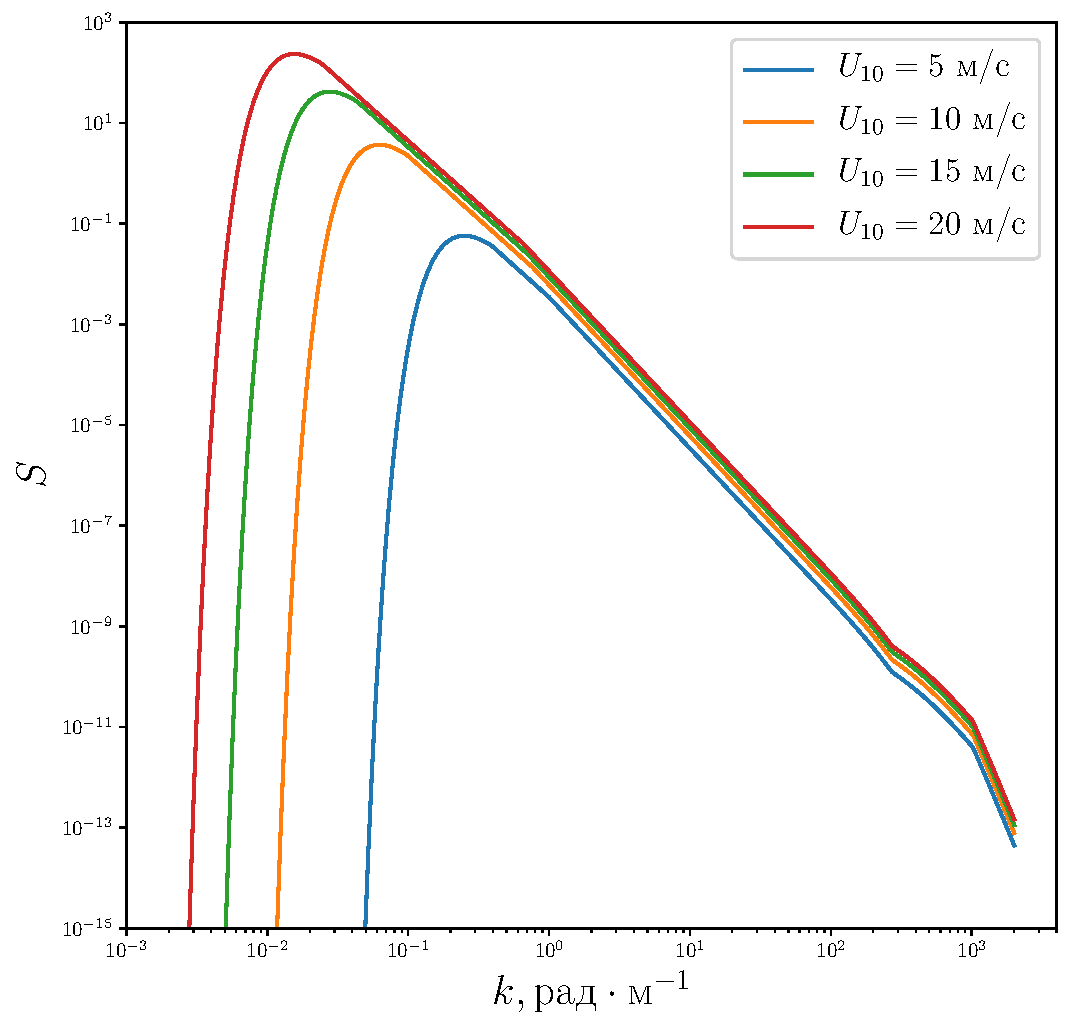
\includegraphics[width=\linewidth]{fig/full_spectrum1.pdf}
			\caption{Спектр высот $S(k)$ при фиксированном значении $\tilde x=20170$ и меняющейся скорости ветра}		
			\label{fig:full_spectrum1}
	\end{minipage}
	\hfill
	\begin{minipage}{0.49\linewidth}
			\centering
			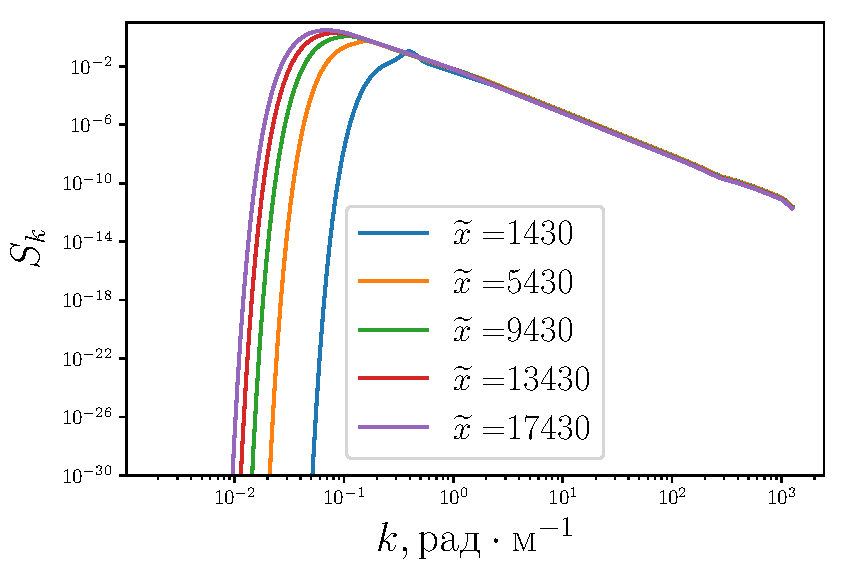
\includegraphics[width=\linewidth]{fig/full_spectrum2.pdf}
			\caption{Спектр высот $S(k)$ при фиксированном значении скорости ветра 
			$U=10$ м/с и меняющемся разгоне}		
			\label{fig:full_spectrum2}
	\end{minipage}
\end{figure}


\begin{figure}[h!]
	\begin{minipage}{0.49\linewidth}
			\centering
			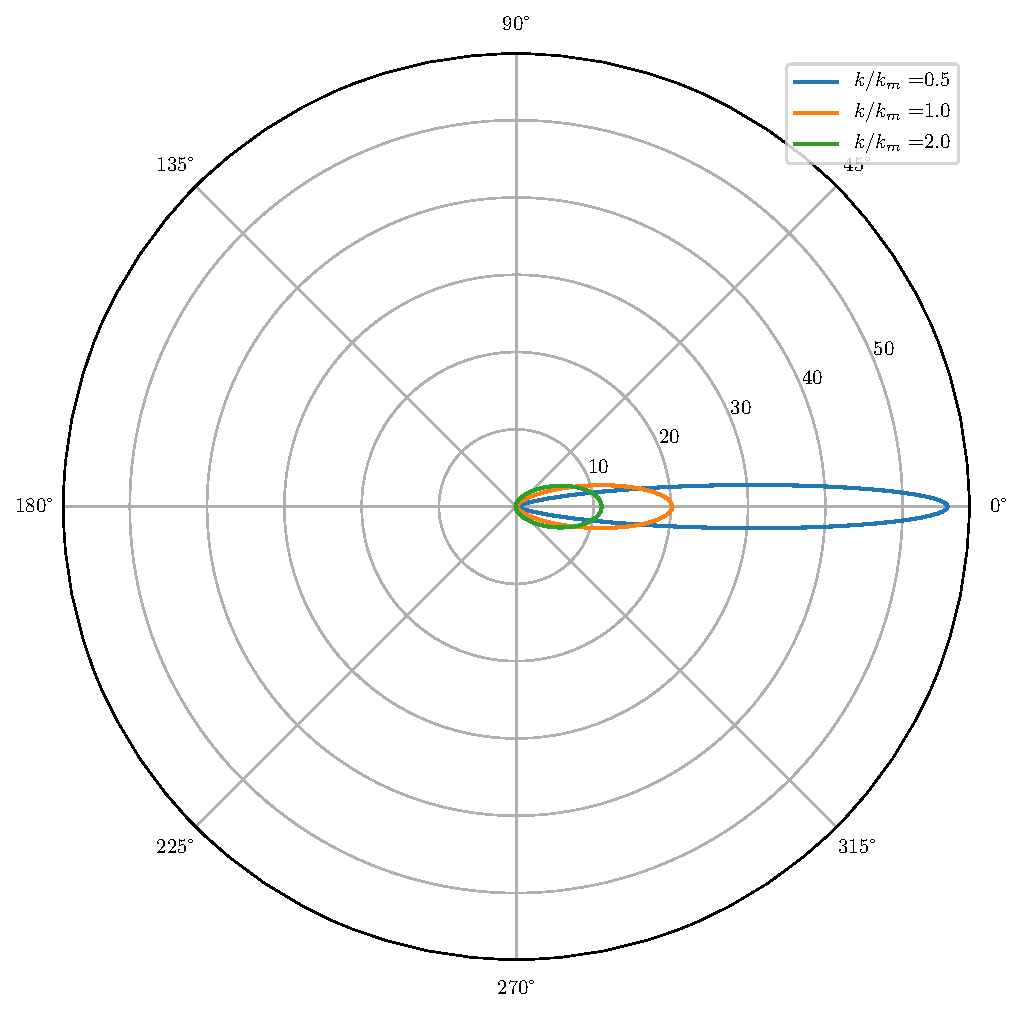
\includegraphics[width=\linewidth]{fig/full_angles1.pdf}	
	\end{minipage}
	\hfill
	\begin{minipage}{0.49\linewidth}
			\centering
			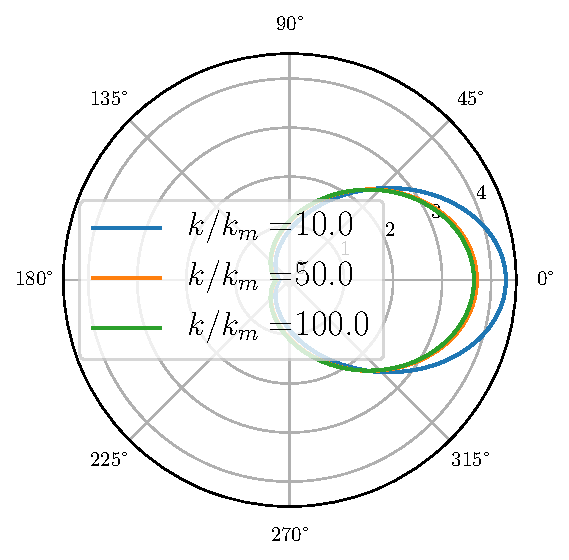
\includegraphics[width=\linewidth]{fig/full_angles2.pdf}
	\end{minipage}
	\caption{Угловое распределение $\Phi_k(\phi)$ в полярных координатах для разных соотношений $k/k_m$}
	\label{fig:full_angles}
\end{figure}


Графики $S_k(k)$ и $\Phi_k(k)$ для наглядности изображены на рис.(\ref{fig:full_spectrum1})-(\ref{fig:full_spectrum2})  и $\ref{fig:full_angles}$ соответственно. Стоит заметить, что число гармоник $N$, используемых для моделирования, прямо пропорционально зависит от скорости ветра. Критерием выбора оптимального числа гармоник стала близость корреляционных функций высот $M$ и наклонов $M_{\theta}$ реального и модельного полей:
\begin{gather*}
	M(\rho)= \int S(k) \cos(k \rho)\dd{k} \\
	\tM(\rho)= \sum_{n=1}^N \frac{A^2_n}{2}\cos(k_n \rho)\\
	M_{\theta}= \int k^2 S(k)\cos(k \rho) \dd{k} \\
	\tM_{\theta}(\rho)=\sum_{n=1}^N \frac{A_n^2}{2} k_n^2 \cos(k_n \rho)
\end{gather*}





Вообще говоря, вместе с [\ref{model}] этого достаточно, чтобы смоделировать поверхностное волнение, но без оптимизации выбора $k_n$ и $\phi_m$ счёт достаточно качественной поверхности будет длиться \sout{до тепловой смерти Вселенной} слишком долго. В данной работе вопрос выбора $\phi_m$ не рассматривается и при моделировании используется равномерный шаг, а вот вопросом выбора $k_n$ мы и зададимся в следующем разделе. 


\subsection{Реальное и модельное поля уклонов и высот волнения}
\begin{figure}[h!]
	\begin{minipage}{0.49\linewidth}
			\centering
			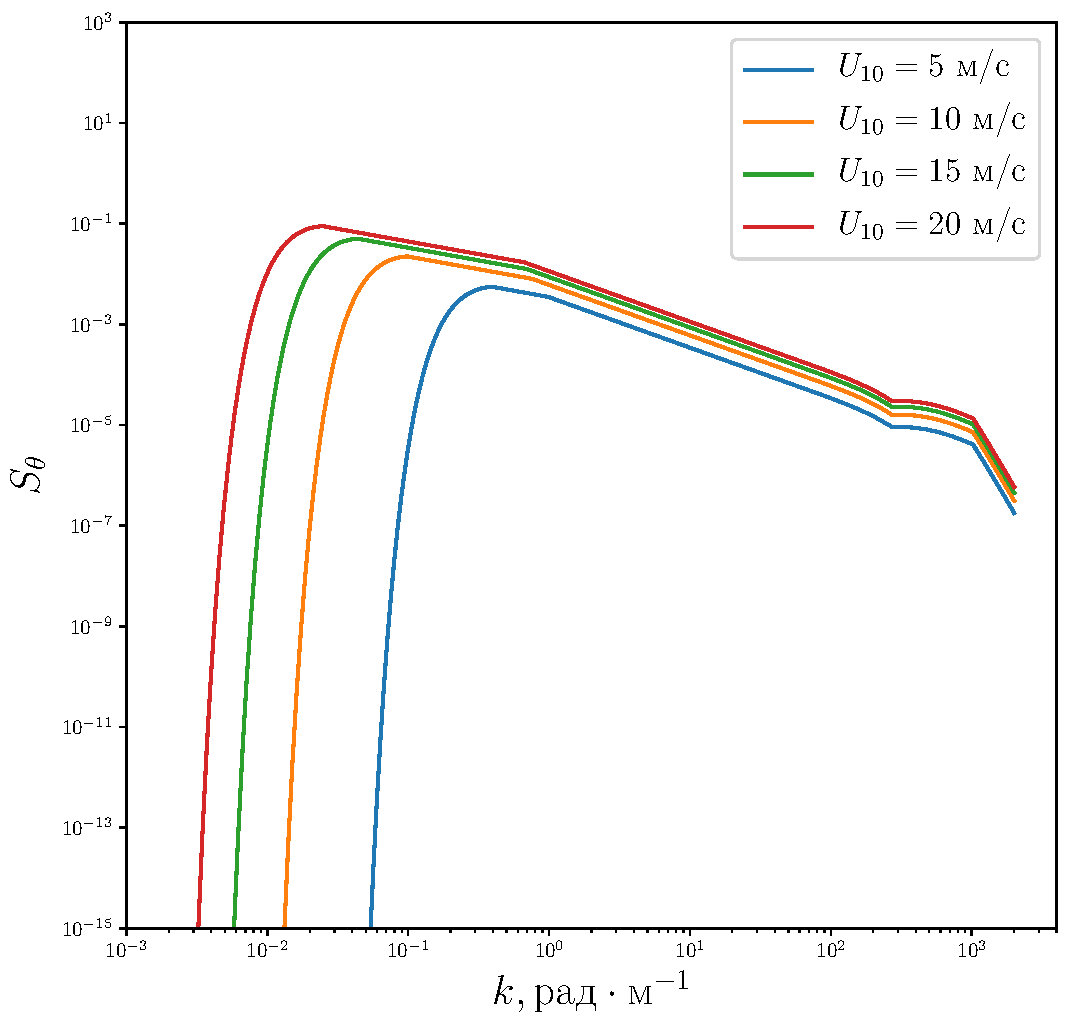
\includegraphics[width=\linewidth]{fig/full_spectrum3.pdf}
			\caption{Спектр наклонов $S_{\theta}(k)$ при фиксированном значении $\tilde x=20170$ и меняющейся скорости ветра}		
			\label{fig:full_spectrum3}
	\end{minipage}
	\hfill
	\begin{minipage}{0.49\linewidth}
			\centering
			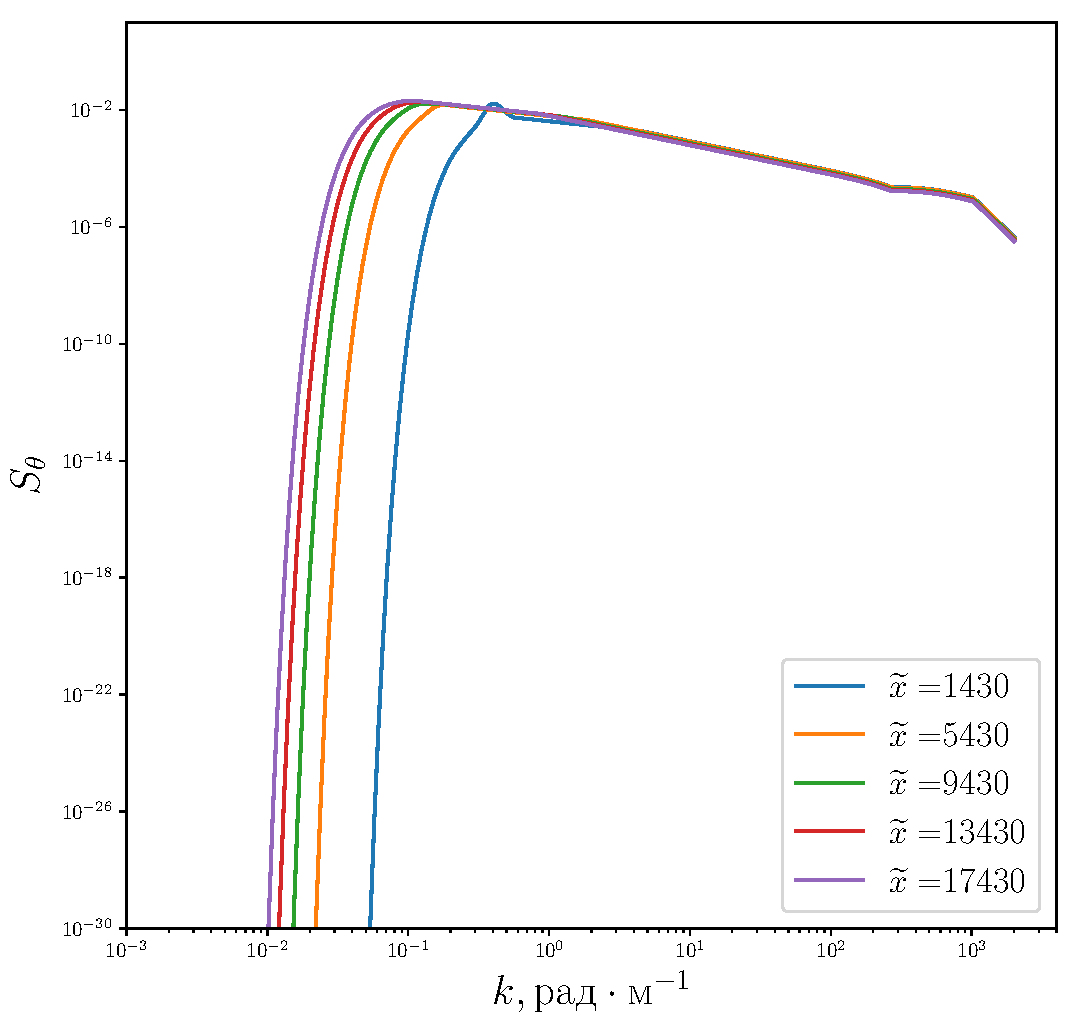
\includegraphics[width=\linewidth]{fig/full_spectrum4.pdf}
			\caption{Спектр наклонов $S_{\theta}(k)$ при фиксированном значении скорости ветра 
			$U=10$ м/с и меняющемся разгоне}		
			\label{fig:full_spectrum4}
	\end{minipage}
\end{figure}
Обратимся сначала к задаче моделирования случайного одномерного поля уклонов взволнованной поверхности. 

Пусть реальное случайное поле уклонов имеет корреляционную функцию $M=\mean {\zeta(r) \zeta(r+\rho)}$, связанную с энергетическим спектром уклонов $S$ соотношением, следующим из (10), (11) при $\phi(\vartheta)=\delta(\vartheta)$:
\begin{equation}
	\label{eq:correlation}
	M(\rho)= \int\limits_0^{\infty} S(k)\cos(k \rho) \dd{k}, 
\end{equation}
Представим модельное поле уклонов в виде суммы N синусоид с детерминированными амплитудами $a_i$ и случайными фазами $\varphi_i$:
\begin{equation}
	\zeta(r)=\sum_{i=1}^N a_i \sin(k_ir+\varphi_i), 
\end{equation}
где фаза $\phi_i$ равномерно распределена в интервале $[0,2\pi]$. Соответствующая этому полю корреляционная функция имеет вид
\begin{equation}
	\widetilde M(\rho)=\sum\limits_{i=1}^N b_i \cos(k_i \rho),
\end{equation}

где $b_i=\frac{a_i^2}{2}$.

Энергетический спектр модельного поля уклонов представляет собой набор дельта-функций, отличных от нуля в узлах $k_i$. Огибающей спектра является кривая, проходящая через точки с абсциссами $k_i$ и ординатами $b_i$. Вопросам определения величин $b_i$ и $k_i$ 
посвящены следующие разделы работы.

Естественным способом размещения $k_i$ будет являться следующий метод:
необходимая область разбивается на $N$ участков одинаковой ширины $\Delta k$, а узлы располагаются в точках $k_i=i \Delta k, i=1,2\dots N$, т.е. эквидистантно.
Амплитуды спектральных составляющих определяются следующим соотношением:
\begin{equation}
	b_i = \int\limits_{(i-1)\Delta k}^{i \Delta k} S(k) \dd{k}
\end{equation}
При этом, из \eqref{eq:correlation} можно заметить, что сумма всех $b_i$ равна дисперсии реального поля
\begin{equation}
	M(0)=\sigma^2=\int\limits_0^{\infty} S(k) \dd{k}
\end{equation}
Однако, при таком способе моделирования корреляционная функция $\tM(\rho)$ является
периодической. Для иллюстрации на рис.(\ref{fig:ca0}) приведены примеры расчёта этой функции для скорости ветра $U=10 \frac{\text{м}}{\text{c}}$ и $N=256$. Конечно, период этой функции может быть удлинён, но это достигается путём увеличения гармоник.
Как видно из рис. \ref{fig:ca05} даже при неразумно большом числе гармоник период корреляционной функции недостаточно большой, что ставит под сомнение применимость такого метода моделирования.

\begin{figure}[h!]
	\begin{minipage}{0.49\linewidth}
			\centering
			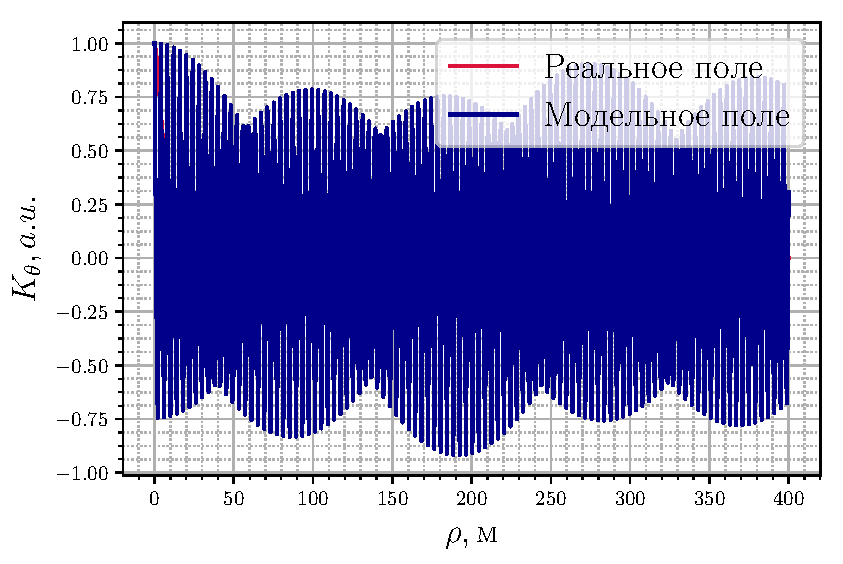
\includegraphics[width=\linewidth]{fig/correlation_height_slopes0.pdf}
			\label{fig:ch0}		
	\end{minipage}
	\hfill
	\begin{minipage}{0.49\linewidth}
			\centering
			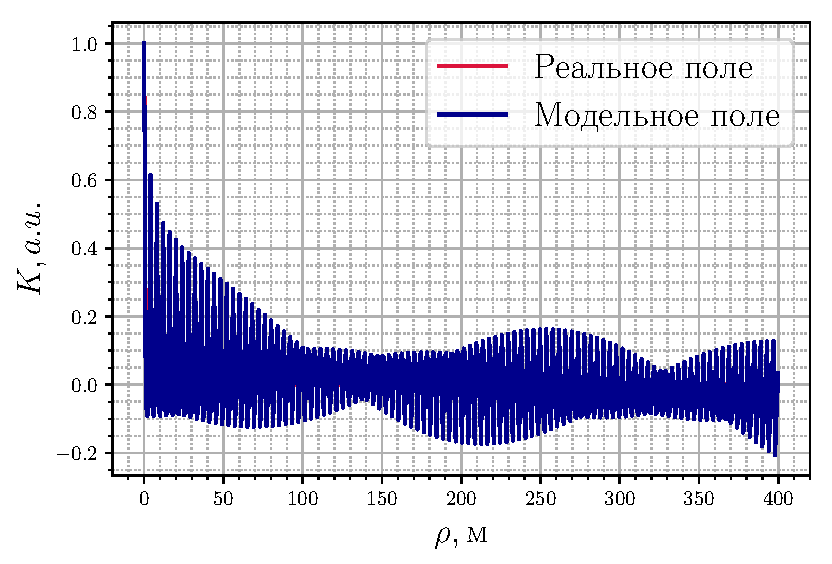
\includegraphics[width=\linewidth]{fig/correlation_angles_slopes0.pdf}
	\end{minipage}
	\caption{Корреляционные функции высот и уклонов при эквидистантном расположении узлов. $U=10 \frac{\text{м}}{c}$, $N=256$}
			\label{fig:ca0}		
\end{figure}

\begin{figure}[h!]
	\begin{minipage}{0.49\linewidth}
			\centering
			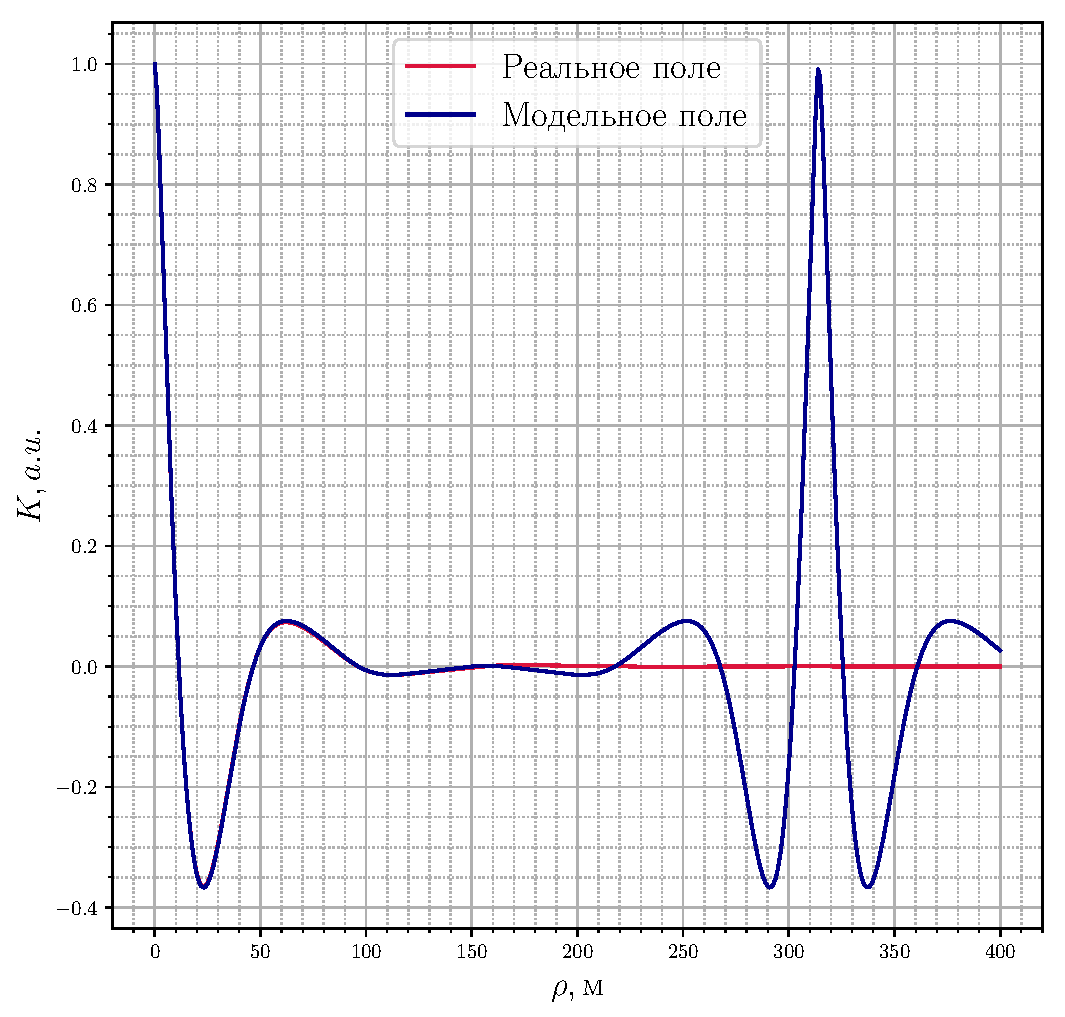
\includegraphics[width=\linewidth]{fig/correlation_height5_slopes2.pdf}
	\end{minipage}
	\hfill
	\begin{minipage}{0.49\linewidth}
			\centering
			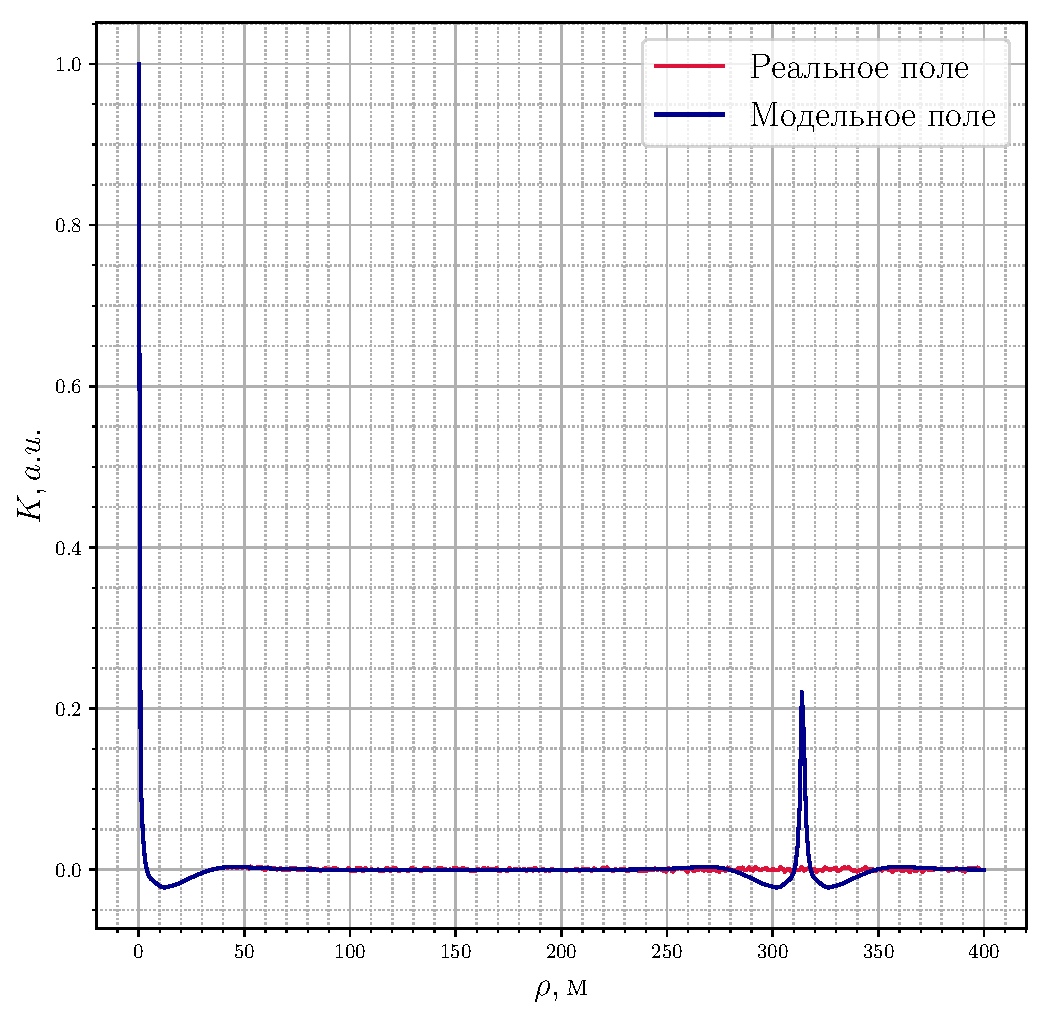
\includegraphics[width=\linewidth]{fig/correlation_angles5_slopes2.pdf}
	\end{minipage}
	\caption{Корреляционные функции высот и уклонов при эквидистантном расположении узлов. $U=10 \frac{\text{м}}{c}$, $N=10^5$}
	\label{fig:ca05}		
\end{figure}
Чтобы функция $\tM(\rho)$ не была периодической, необходимо лишь неэквидистантно расположить узлы $k_i$ на оси частот. Например, можно использовать различные детерминированные способы расположения узлов на оси частот.

Поскольку спектр частот (см. рис. \ref{fig:full_spectrum1}) удобно представим в логарифмическом масштабе, то можно располагать узлы эквидистантно в логарифмическом масштабе. Очевидно, что такой способ значительно лучше, чем первый способ. Функция корреляции высот довольно быстро сходится к функции реального поля. С функцией корреляции наклонов проблем возникает больше, поскольку она быстро принимает шумовой характер.

\begin{figure}[h!]
	\begin{minipage}{0.49\linewidth}
			\centering
			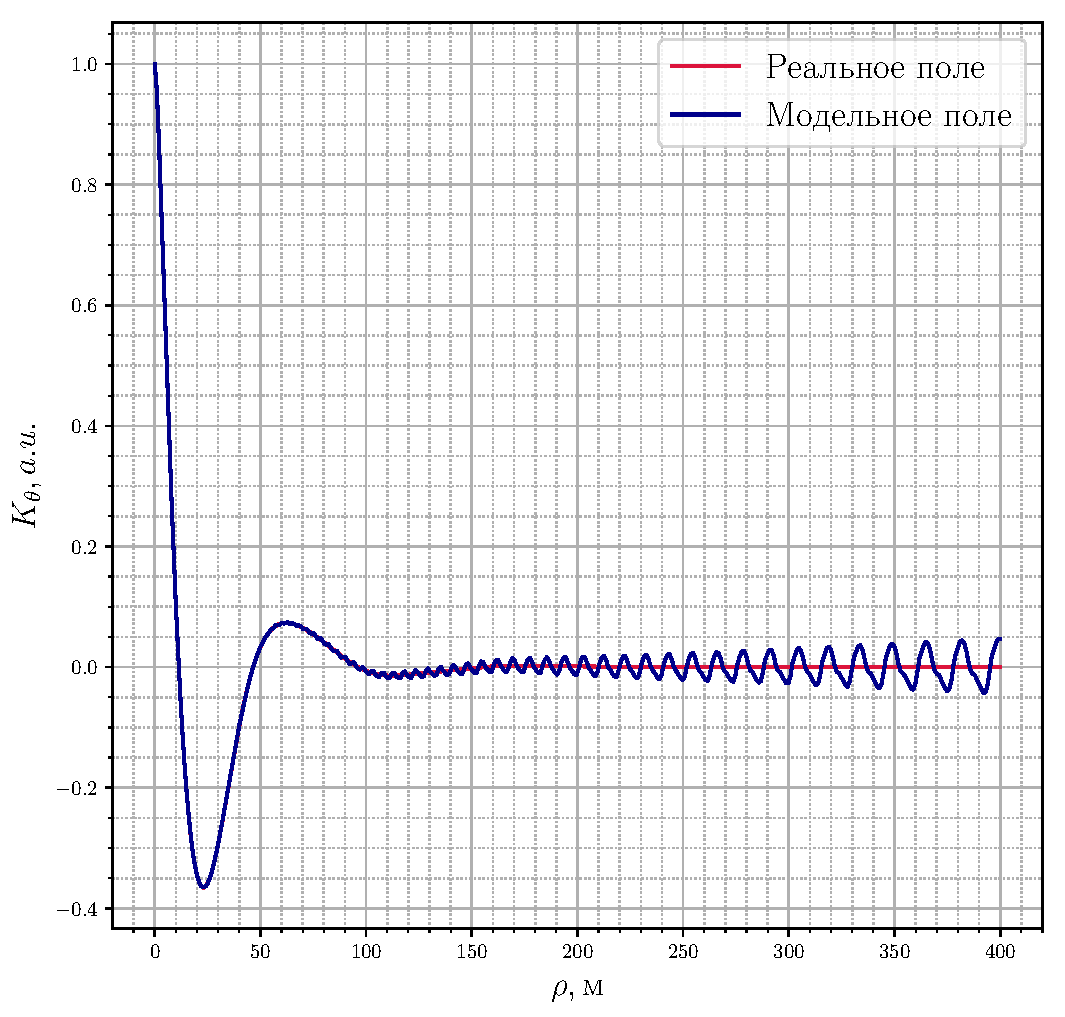
\includegraphics[width=\linewidth]{fig/correlation_height_slopes1.pdf}
			\label{fig:ch1}		
	\end{minipage}
	\hfill
	\begin{minipage}{0.49\linewidth}
			\centering
			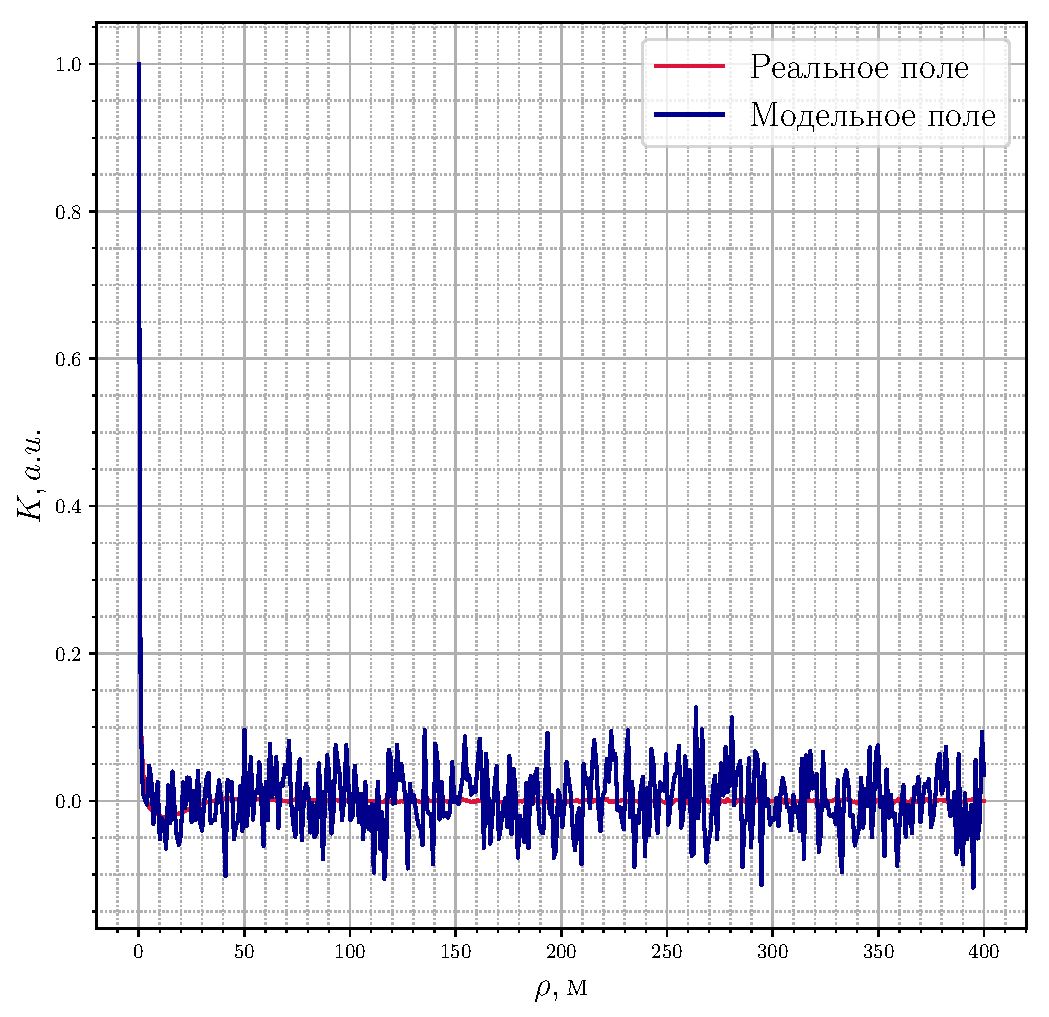
\includegraphics[width=\linewidth]{fig/correlation_angles_slopes1.pdf}
			\label{fig:ca1}		
	\end{minipage}
	\caption{Корреляционные функции высот и уклонов при логарифмическом расположении узлов. $U=10 \frac{\text{м}}{c}$, $N=256$}
\end{figure}



Очевидно, что способов выбора узлов по детерминированному закону существует бесконечно много, но наилучшими следует считать те способы, которые обеспечивают наименьший уровень <<шума>> на <<хвосте>> корреляционной функции $\tM(\rho)$.

\subsubsection{Метод <<отбеливания>> спектра}
Допустим что величины $k_i$ не находятся в дробно-рациональных отношениях друг к другу. В этом случае можно полагать, что сложение гармонических составляющих с частотами $k_i$ и амплитудами $b_i$ при больших $\rho$ происходит <<некогерентным>> образом. При этом мощность <<шума>> функции $\tM(\rho)$ определяется выражением 
$\displaystyle \sigma^2= \sum_{i=1}^N \frac{b_i^2}{2}$. В области малых $\rho$, напротив, гармоники суммируются <<когерентно>> и соответствующая <<мощность>> равна 
$\displaystyle \tM^2(0)=\qty(\sum_{i=1}^N b_i)^2$. Образуем величину 

\begin{equation}
	\label{eq:Q}
	Q=\sigma^2/\tM(0)
\end{equation}, которая характеризует относительную мощность шумов. Минимум этой величины находится путём решения системы уравнений $\pdv{Q}{b_i}=0$, для $i=1,2,\dots,N.$
Результатом её решения является $b_1=b_2=\dots = d_N$. Спектр модельного поля при этом имеет близкий к белому вид, а выравнивание амплитуд спектральных компонент реального поля $S(k)$ сводится к разбиению области определения спектра $[0, k_m]$ на участки $\Delta k_i$, интегралы по которым от функции $S(k)$ имеют одно и то же значения $b_i=b_0=\sigma^2/N$.

\begin{figure}[h!]
	\begin{minipage}{0.49\linewidth}
			\centering
			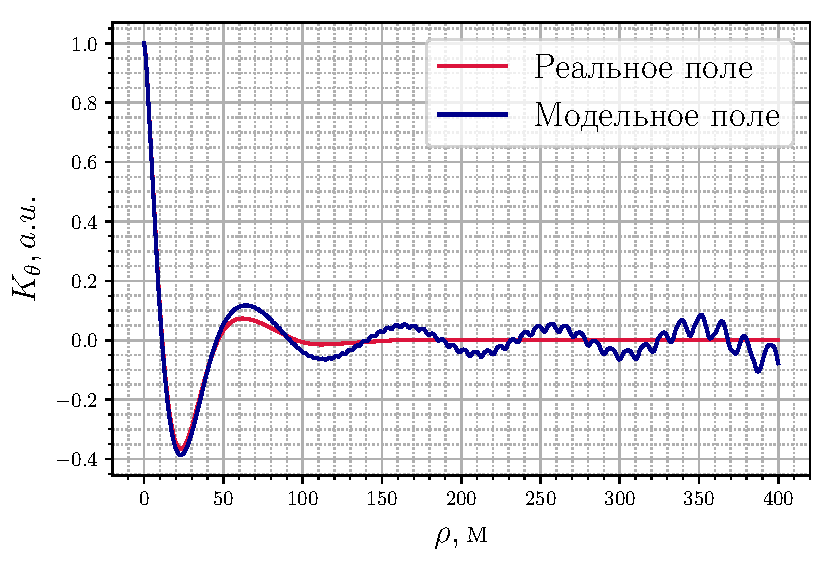
\includegraphics[width=\linewidth]{fig/correlation_height_slopes2.pdf}
			\label{fig:ch21}		
	\end{minipage}
	\hfill
	\begin{minipage}{0.49\linewidth}
			\centering
			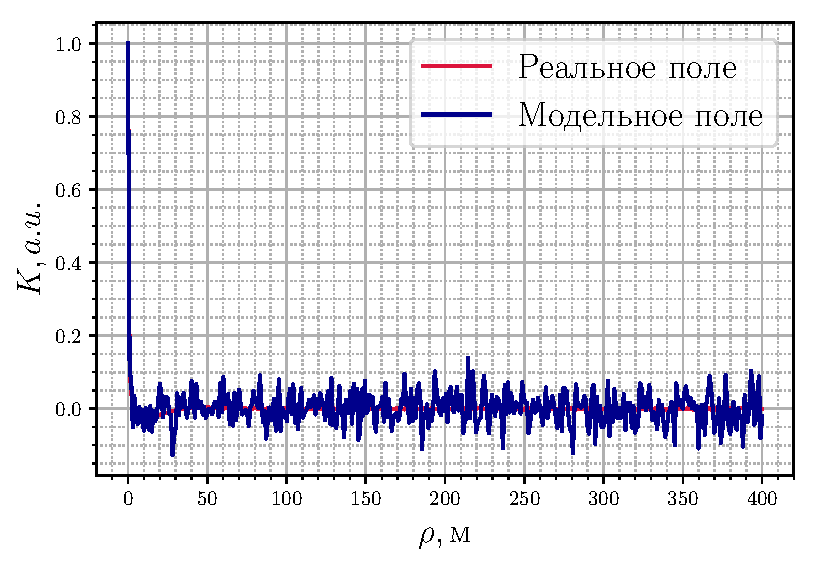
\includegraphics[width=\linewidth]{fig/correlation_angles_slopes2.pdf}
	\end{minipage}
	\caption{Корреляционные функции высот и уклонов при расположении узлов по методу <<отбеливания>> спектра для уклонов. $U=10 \frac{\text{м}}{c}$, $N=256$}
			\label{fig:ca21}		
\end{figure}


\begin{figure}[h!]
	\begin{minipage}{0.49\linewidth}
			\centering
			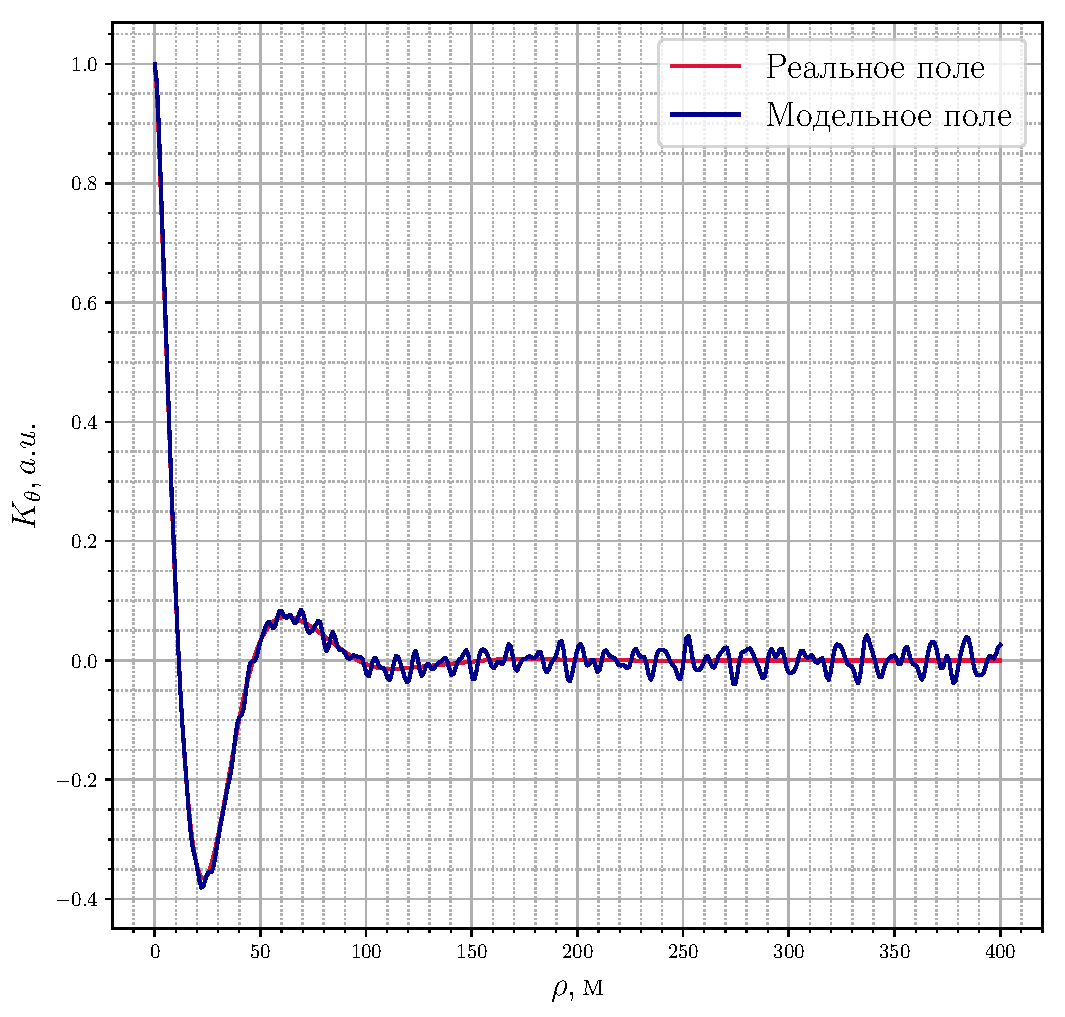
\includegraphics[width=\linewidth]{fig/correlation_height_height2.pdf}
			\label{fig:ch22}		
	\end{minipage}
	\hfill
	\begin{minipage}{0.49\linewidth}
			\centering
			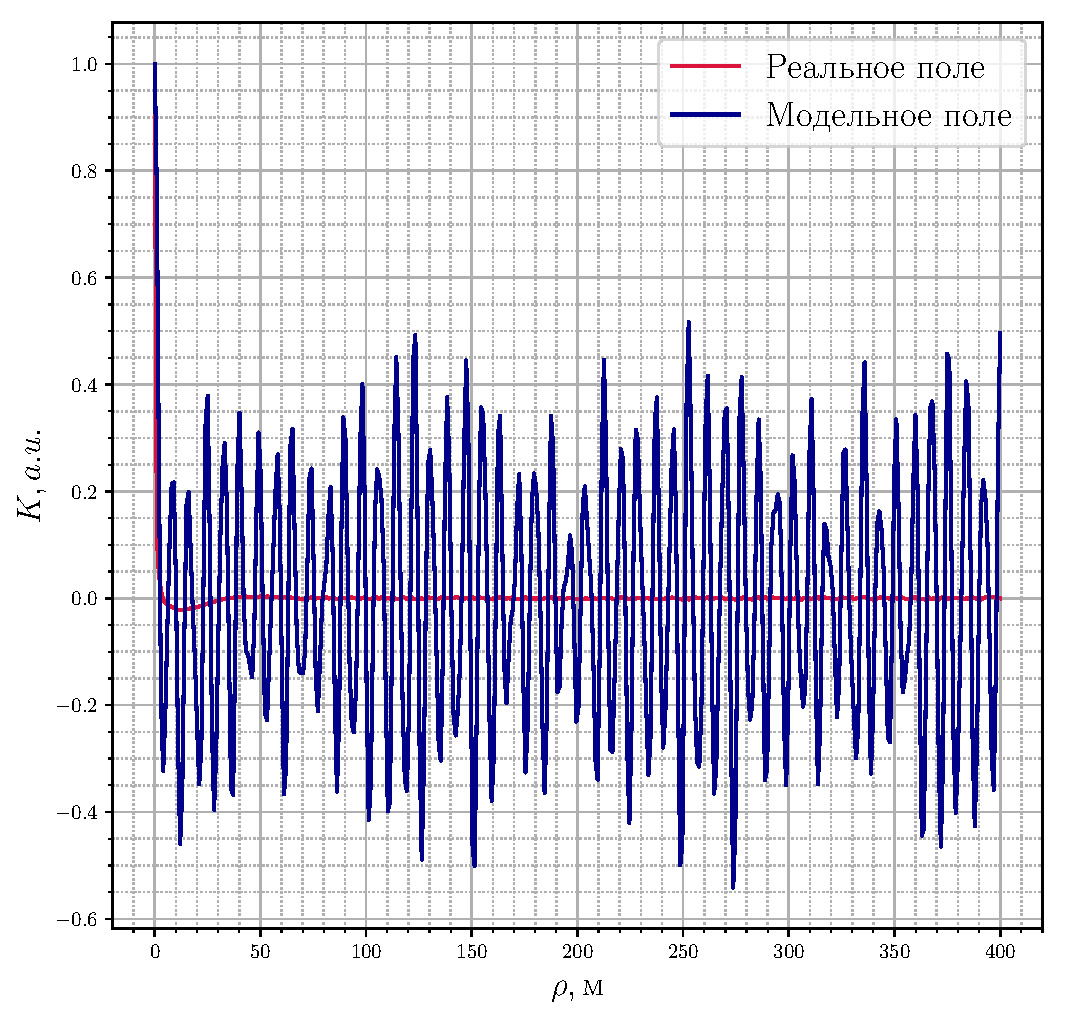
\includegraphics[width=\linewidth]{fig/correlation_angles_height2.pdf}
	\end{minipage}
	\caption{Корреляционные функции высот и уклонов при расположении узлов по методу <<отбеливания>> спектра для высот. $U=10 \frac{\text{м}}{c}$, $N=256$}
			\label{fig:ca22}		
\end{figure}

Заметим теперь, что, рассуждая о способах разбиения интервала частот $[0, k_m]$ на участки $\Delta k_i$, мы оставляли нерешенным вопрос о выборе собственно узлов спектра $k_i$ внутри этих участков. Обычно узел $k_i$ ставится у правой границы ячейки $\Delta k_i$. При этом, однако, оказывается, что модельная корреляционная функция плохо согласуется с реальной корреляционной функцией в области малых $\rho$. Для достижения такого согласия следует потребовать сопряжения всех производных (от первого до $N$-го порядка) функций $\tM(\rho)$ и $M(q)$ при $\rho=0$. Это условие эквивалентно требованию сопряжения моментов спектров модельного и реального полей, которое записывается в виде 
\begin{equation}
	\sum_{i=1}^N b_ik_i^{2p}=\int\limits_{0}^{\infty} k^{2p}S\dd{k},
\end{equation}
для $p=1,2,\dots,N.$

Полученная система N уравнений для N неизвестных $k_i$ не имеет общего решения и потому может анализироваться лишь численно, что тоже связано со значительными сложностями.



Наиболее простое решение вопроса о выборе узлов заключается в том, чтобы потребовать выполнения облегченного, по сравнению с предыдущим, условия сопряжения вторых моментов модельного и реального спектров высот:
\begin{equation}
	b_i k_i^2=\int\limits_{\Delta k_i} k^2 S(k)  \dd{k}.
\end{equation}

Из него непосредственно следует правило нахождения узлов $k_i$. В частности, получаем
\begin{equation}
	k_i=\sqrt\frac{1}{b_0} \int\limits_{\Delta k_i} k^2 S \dd{k}.
\end{equation}

Такой способ выбора узлом, как нетрудно убедиться, обеспечивает сопряжения корреляционных функция реального и модельного полей по второй производной в нуле, или, иначе говоря, равенство дисперсий кривизн этих полей. 




Стоит сказать, что весь этот раздел был написан для поля высот $S(k)$. Но те же рассуждения можно провести и для поля наклонов $S_{\theta}(k)$, которое связано с полем высот соотношением $S_{\theta}=k^2 S(k)$. Таким образом, положив 
\begin{equation}
	S(k)\longrightarrow k^2 S(k)
\end{equation}
мы можем получить уравнения для моделирования поля наклонов. 

На рис. \ref{fig:ca21} и \ref{fig:ca22} построены графики зависимости корреляционных функций высот и уклонов для метода <<отбеления>> спектра, примененного соответственно для наклонов и высот. Нетрудно заметить, что этот метод лучше предыдущих работает для одной выбранной функции, но с другой вызывает проблемы. Это особенно заметно на рис. \ref{fig:ca22}: поле высот $\tM$ хорошо сходится к реальному полю $M$, но $\tM_{\theta}$ очень далека от реальной. 

\newpage
\section{Заключение}


\begin{figure}[h!]
\begin{minipage}[h]{0.45\linewidth}
	\centering
	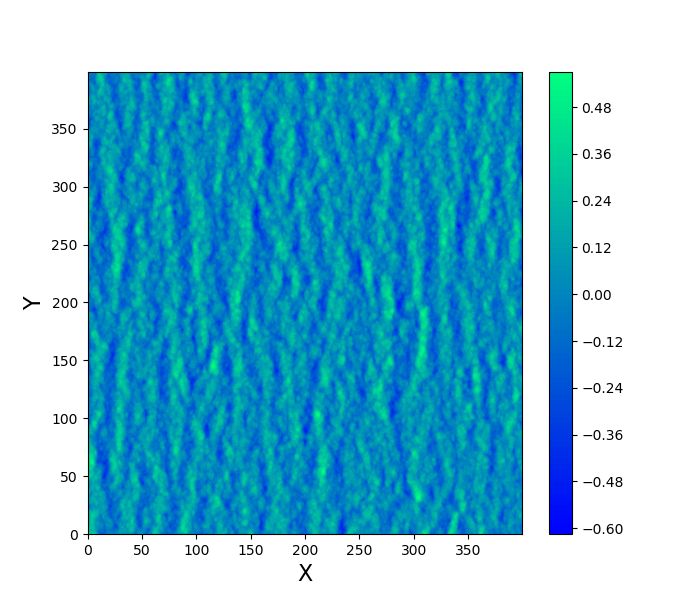
\includegraphics[width=\linewidth]{img/water5.png}
	\caption{Моделирование высот морского волнения. $N=256, ~ U_{10}=5$ }
	\label{fig:water5}
\end{minipage}
\hfill
\begin{minipage}[h]{0.45\linewidth}
	\centering
	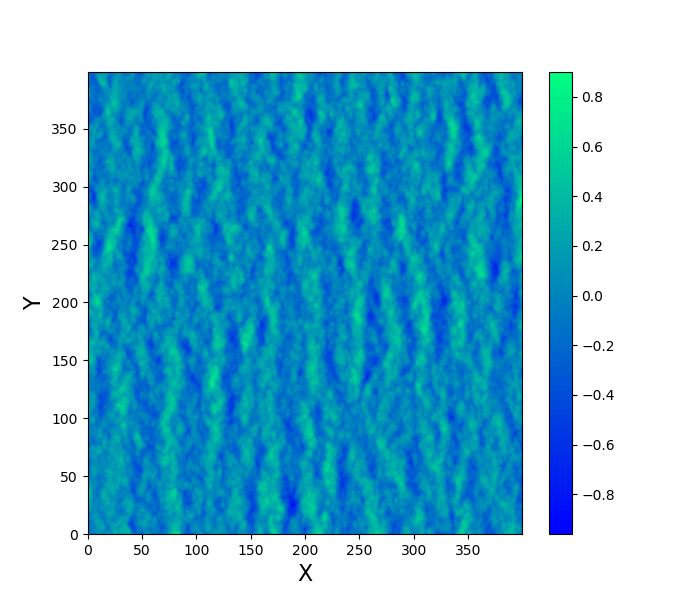
\includegraphics[width=\linewidth]{img/water6.png}
	\caption{Моделирование высот морского волнения. $N=256, ~ U_{10}=6$ }
	\label{fig:water6}
\end{minipage}

\vfill
\begin{minipage}[h]{0.45\linewidth}
	\centering
	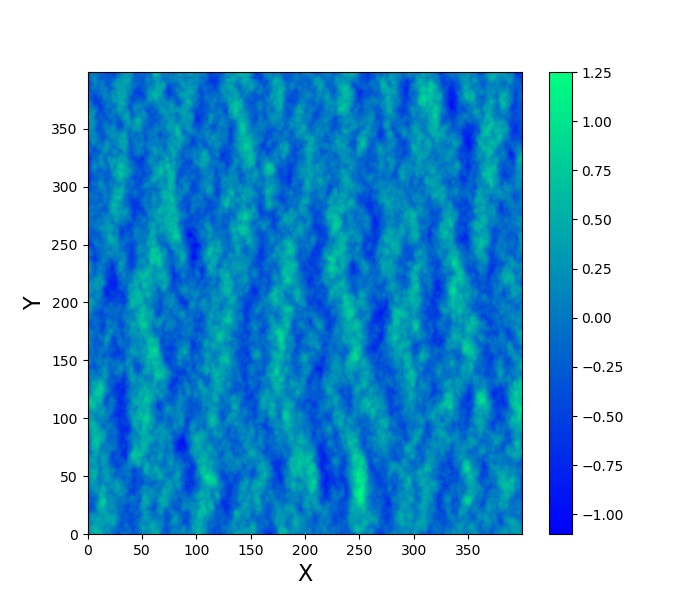
\includegraphics[width=\linewidth]{img/water7.png}
	\caption{Моделирование высот морского волнения. $N=256, ~ U_{10}=7$  }
	\label{fig:water7}
\end{minipage}
\hfill
\begin{minipage}[h]{0.45\linewidth}
	\centering
	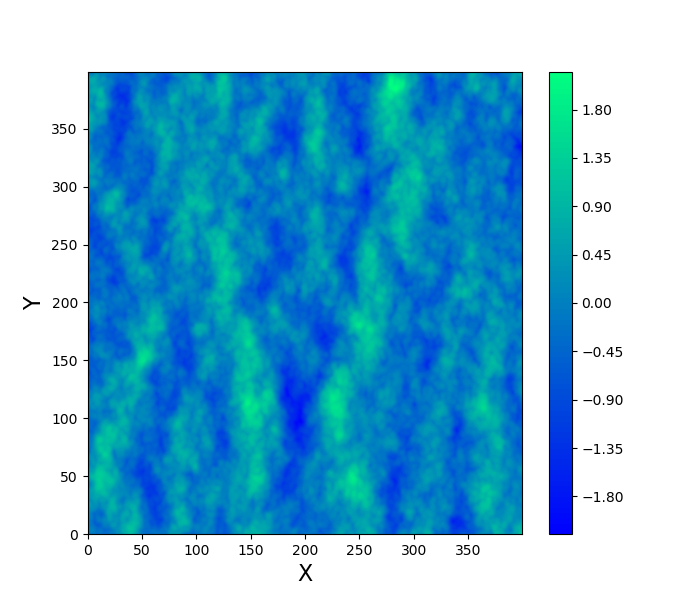
\includegraphics[width=\linewidth]{img/water10.png}
	\caption{Моделирование высот морского волнения. $N=256, ~ U_{10}=10$ }
	\label{fig:water10}
\end{minipage}
\end{figure}


На рисунках \ref{fig:water5}-\ref{fig:water10} представлены 
смоделированные  поля высот для разных скоростей ветра\footnote{Модель написала на языке Python с использованием библиотек NumPy и SciPy, отчёт по практике и презентация к ней оформлены в издательской системе \LaTeX\,с использованием пакета Beamer. Актуальную версию программы можно найти на 
Github'e: 
\begin{center}
\qrcode{https://github.com/KirillPonur/water}
\end{center}}. В дальнейшем планируется усовершенствовать выбор азимутальных координат $\phi$, а также выбором некой новой величины $Q$ (см.\eqref{eq:Q}) добиться сопряжения метода <<отбеливания>> спектра для наклонов и высот. 
% 

\appendix
\section{Приложение}
\label{model}
\subsection{Модель спектра волнения}

Для моделирования волнения используется следующая модель спектра волнения, предложенного в \cite{Karaev2}: 
\begin{equation}
	\label{eq:Sw}
	\begin{cases}
		S(\omega)=S_J(\omega), &  0<\omega\leq 1.2\,\omega_m\\
		S(\omega)= \frac{\alpha_2}{\omega^4}, &  1.2 \,\omega_m < \omega \leq \alpha_m \omega_m\\
		S(\omega)= \frac{\alpha_3}{\omega^5}, &   \alpha_m \omega_m< \omega \leq \omega_gk\\
		S(\omega)= \frac{\alpha_4}{\omega^{2.7}}, & \omega_{gk}<\omega\leq \omega_h\\
		S(\omega)= \frac{\alpha_5}{\omega^5}, & \omega_h<\omega,
	\end{cases}
\end{equation}
где коэффициенты $\alpha_i$ задаются следующим образом:
\begin{equation}
	\label{eq:alpha_i}
	\begin{cases}
		\alpha_2=S_J(1.2 \omega_m)\cdot (1.2 \omega_m)^4 \\
		\alpha_3=a_2\cdot \alpha_m \omega_m \\
		\alpha_4= \frac{\alpha_3}{\omega^{2.3}_{gk}} \\
		\alpha_5 = \alpha_4 \cdot \omega_h^{2.3} \\
		\alpha_m = f(U_{10}), & 
	\end{cases}
\end{equation}
$U_{10} \text{-- скорость ветра на высоте 10 метров над уровнем моря,}$ а $S_J(\omega)$-- спектр JONSWAP:
\begin{equation}
\label{eq:Sj}
	S_J(\omega)\sim \frac{g^2}{\omega^{5}}\exp{-\qty(\frac{\omega_m}{\omega})^4}
	\cdot \gamma^{\exp{-\omega^2}}
\end{equation}
Стоит отметить, что в конечном счете формулы \eqref{eq:Sw},\eqref{eq:alpha_i},\eqref{eq:Sj} в модели использовались в $k-$представлении, т.е.  был выполнен переход $S(\omega)\rightarrow S(k)$


\subsection{Модель углового распределения}
Угловое распределение $\Phi_{\omega}$ в данной работе описывается следующей формулой:
\begin{equation}
	\Phi_{k} (k, \phi)= A\cdot \cosh^{-1}{2B(k) \phi}, ~~ -\pi\leq \phi \leq \pi,
\end{equation}
где $\phi=\phi_m = \phi_w$, $\phi_w$-- генеральное направление распространения волнения,
$\phi_m$-- текущий азимутальный угол, $A$-- нормировочный коэффициент.




Дисперсионное уравнение в данной работе имеет вид:
\begin{equation}
	\label{eq:w_k}
	\omega(k)=\sqrt{gk+a\cdot k^3},
\end{equation}
% Значения и физический смысл всех коэффициентов можно найти в \cite{Karaev1}, а также в исходном коде программы 
% (\href{https://github.com/KirillPonur/water}{github.com/KirillPonur/water})

\newpage
\begin{thebibliography}{}
	\bibitem{Rytov} \textit{С.М. Рытов}, Введение в статистическую радиофизику // Изд. 2-е, перераб. и доп. - Москва : Наука, 1976. - Ч. 1. Случайные процессы \S\S 14-18, 38-42 
	\bibitem{Karaev1} \textit{В.Ю.Караев, М.Б. Каневский, Г.Н. Баландина}, Численное моделирование поверхностного волнения и дистанционное зондирование // Препринт №552 ИПФ РАН, 2002, С.1-10.
	\bibitem{Veber} \textit{В.Л. Вебер}, О моделировании случайного профиля морской поверхности // Изв. вузов. Радиофизика. 2017. Т. 60, № 4. С. 346.
	\bibitem{Karaev2} \textit{В.Ю.Караев, Г.Н. Баландина} Модифицированный спектр волнения и дистанционное зондирование // Исследование Земли из космоса, 2000, N5, C.1-12.
	\bibitem{Longe} \textit{М.С. Лонге-Хиггинс} Статистический анализ случайной движущейся поверхности // в кн.: Ветровые волны, М.: Иностранная наука, 1962, С.112-230
\end{thebibliography}



\end{document}